%% LaTeX_Thesis_Template.tex
% An unofficial LaTeX template for Cranfield theses.
% 2017/08/14 Daniel Auger's unofficial Cranfield thesis .sty file
% 2023/05/31 Updated by Shaun Forth (SAF) for logo inclusion
% 2023/06/08 SAF removed capitalisation on title pages on advice of Amy 
% Greenaway and Alison Waters. Added Daniel Auger's headers with 
% chapter and section names.
% 2023/06/08 SAF simplified logo inclusion

%%
% This document is an example of the use of the unofficial "cranfieldthesis" 
% LaTeX style file.  I hope it's useful, and a good likeness of the Word template.

\documentclass[12pt,oneside]{book} % for one-sided printing
%\documentclass[12pt,twoside]{book} % for two-sided printing

% Use the custom "cranfieldthesis" LaTeX style file. 
\usepackage{cranfieldthesis}
\usepackage{lscape} % for landscape pages
\usepackage{amsmath}
\usepackage{enumitem}
\usepackage{changepage}
\usepackage{pdfpages}
\usepackage{blindtext}% Just used so we can generate some example text
\usepackage{algorithm}
\usepackage{algpseudocode}
\usepackage{amssymb}
\usepackage{mathtools}
\usepackage[export]{adjustbox}
\usepackage{lipsum}
\usepackage{booktabs}  % For better quality tables
\usepackage{siunitx}
\usepackage{float}
\usepackage{longtable} % Pour les tableaux sur plusieurs pages
\usepackage{tabularx}  % for the X column type
\usepackage{listings}
\usepackage{xcolor}
\usepackage{caption}
\usepackage{xfrac}
\usepackage{indentfirst}
\usepackage{subcaption}
\usepackage{graphicx}
\usepackage{geometry}
\usepackage{titlesec}
\geometry{a4paper, margin=1in}
\hypersetup{
    colorlinks,
    linkcolor={blue!50!blue},
    citecolor={blue!50!blue},
    urlcolor={blue!80!blue}
}

% By default, LaTeX uses a serif font - these are traditionally thought to be
% easier to read.   If you'd prefer sans-serif, please uncomment the 
% following line.
% \renewcommand{\familydefault}{\sfdefault}

% Example parameters for a typical taught MSc course
\title{Future Position Prediction for Pressure Refuelling Port
    of Commercial Aircraft}
\author{Alexis Balayre}
\date{May 2024}
\school{\SATM}
\course{Computational and Software Techniques in Engineering}
\degree{MSc}
\academicyear{2023--2024}
\setCUPartnerLogo{logo-airbus.png}
\supervisors{Dr Boyu Kuang and Dr Stuart Barnes}
\copyrightyear{2024}

% References
% Cranfield Numbered Style
\usepackage[numbers]{natbib} % for nice referencing
\makeatletter % Reference list option change to number and period
\renewcommand\@biblabel[1]{#1.} % from [1] to 1
\makeatother %

\begin{document}

%% Front matter
%
% This is where we do the title page, etc.
%

\frontmatter

% Standard-Form Title Pages
\maketitle

% Abstract and Keywords
\begin{abstract}
    Replace with your abstract text of not more than 300 words.
\end{abstract}

\begin{keywords}
    Replace with at least 6, semicolon seperated keywords (not contained within the thesis title) – this makes the thesis searchable.
\end{keywords}

% Acknowledgements
\chapter{Acknowledgements}
The author would like to thank \dots

% Use single spacing for Table of Contents, List of Figures, etc
{
    \clearpage

    % Table of Contents
    \singlespacing{
        \tableofcontents
    }
    \clearpage

    % List of Figures
    \listoffigures

    \clearpage
    % List of Tables
    \listoftables
}

% The list of abbreviations can't be automatically generated so you need to populate it yourself
\begin{listofabbreviations}
    \abbrev{ML}{Machine Learning}
    \abbrev{DL}{Deep Learning}
    \abbrev{AI}{Artificial Intelligence}
    \abbrev{CNN}{Convolutional Neural Network}
    \abbrev{RNN}{Recurrent Neural Network}
    \abbrev{LSTM}{Long Short-Term Memory}
    \abbrev{GRU}{Gated Recurrent Unit}
    \abbrev{EKF}{Extended Kalman Filter}
    \abbrev{AAGR}{Autonomous Aircraft Ground Refueling}
    \abbrev{AGR}{Aircraft Ground Refueling}
    \abbrev{UAV}{Unmanned Aerial Vehicle}
    \abbrev{AAR}{Autonomous Aerial Refueling}
    \abbrev{DGPS}{Differential Global Positioning System}
    \abbrev{SVM}{Support Vector Machine}
    \abbrev{HOG}{Histogram of Oriented Gradients}
    \abbrev{SOTA}{State-of-the-Art}
    \abbrev{AIS}{Automatic Identification System}
    \abbrev{GPS}{Global Positioning System}
\end{listofabbreviations}

%% Main Matter
%
% This is where we include the main thesis content.
%
\mainmatter\pagestyle{fancy}
\fancyhead[L]{\nouppercase{\leftmark}}
\fancyhead[R]{\nouppercase{\rightmark}}

%%%%%%%%%%%%%%%%%%%%%%%%%%%%%%%%%%%%%%%%%%%%%%%%%%%%%%%%%%%%%%%%%%%%%%%%%%%%%%%%
%%%%%%%%%%%%%%%%%%%%%%%%%%%%%%%%% INTRODUCTION %%%%%%%%%%%%%%%%%%%%%%%%%%%%%%%%%
\chapter{Introduction}
Ground pressure refuelling is a standard method used to refuel commercial
aircraft safely and efficiently. This process involves using a hydrant system,
which consists of underground fuel pipelines connected to a network of fuel
hydrants located at aircraft parking positions~\cite{blakey2011aviation}. The
hydrant system is supplied with fuel from storage tanks, typically located near
the airport~\cite{kazda2015airport}.

When an aircraft is ready for refueling, a hydrant dispenser vehicle, also
known as a hydrant truck or cart, is connected to the hydrant pit using a
flexible hose~\cite{sati2019aircraft}. The hydrant dispenser vehicle is
equipped with a pressure control valve, a flow meter, and a filtration system
to ensure that the fuel meets the required quality
standards~\cite{iata2019guidance}.

The refueling process begins by connecting the hydrant dispenser vehicle to the
aircraft's fuel panel using another flexible hose~\cite{sati2019aircraft}. The
pressure control valve on the hydrant dispenser vehicle is then used to
regulate the fuel pressure and flow rate, ensuring that the fuel is delivered
to the aircraft at the appropriate pressure and volume~\cite{iata2019guidance}.

One of the main advantages of pressure ground refueling is its efficiency. This
method allows for high fuel flow rates, which can significantly reduce aircraft
turnaround times~\cite{blakey2011aviation}. Additionally, the use of
underground pipelines eliminates the need for fuel trucks, reducing traffic
congestion and the risk of accidents on the apron~\cite{kazda2015airport}.

Safety is another critical aspect of pressure ground refueling. The hydrant
system is designed with multiple safety features, such as emergency shutdown
valves and leak detection systems, to minimise the risk of fuel spills and
fires~\cite{iata2019guidance}. Moreover, the hydrant dispenser vehicles are
equipped with safety devices, such as dead man switches and bonding cables, to
prevent incidents during the refueling process~\cite{sati2019aircraft}.

\begin{figure}[H]
    \centering
    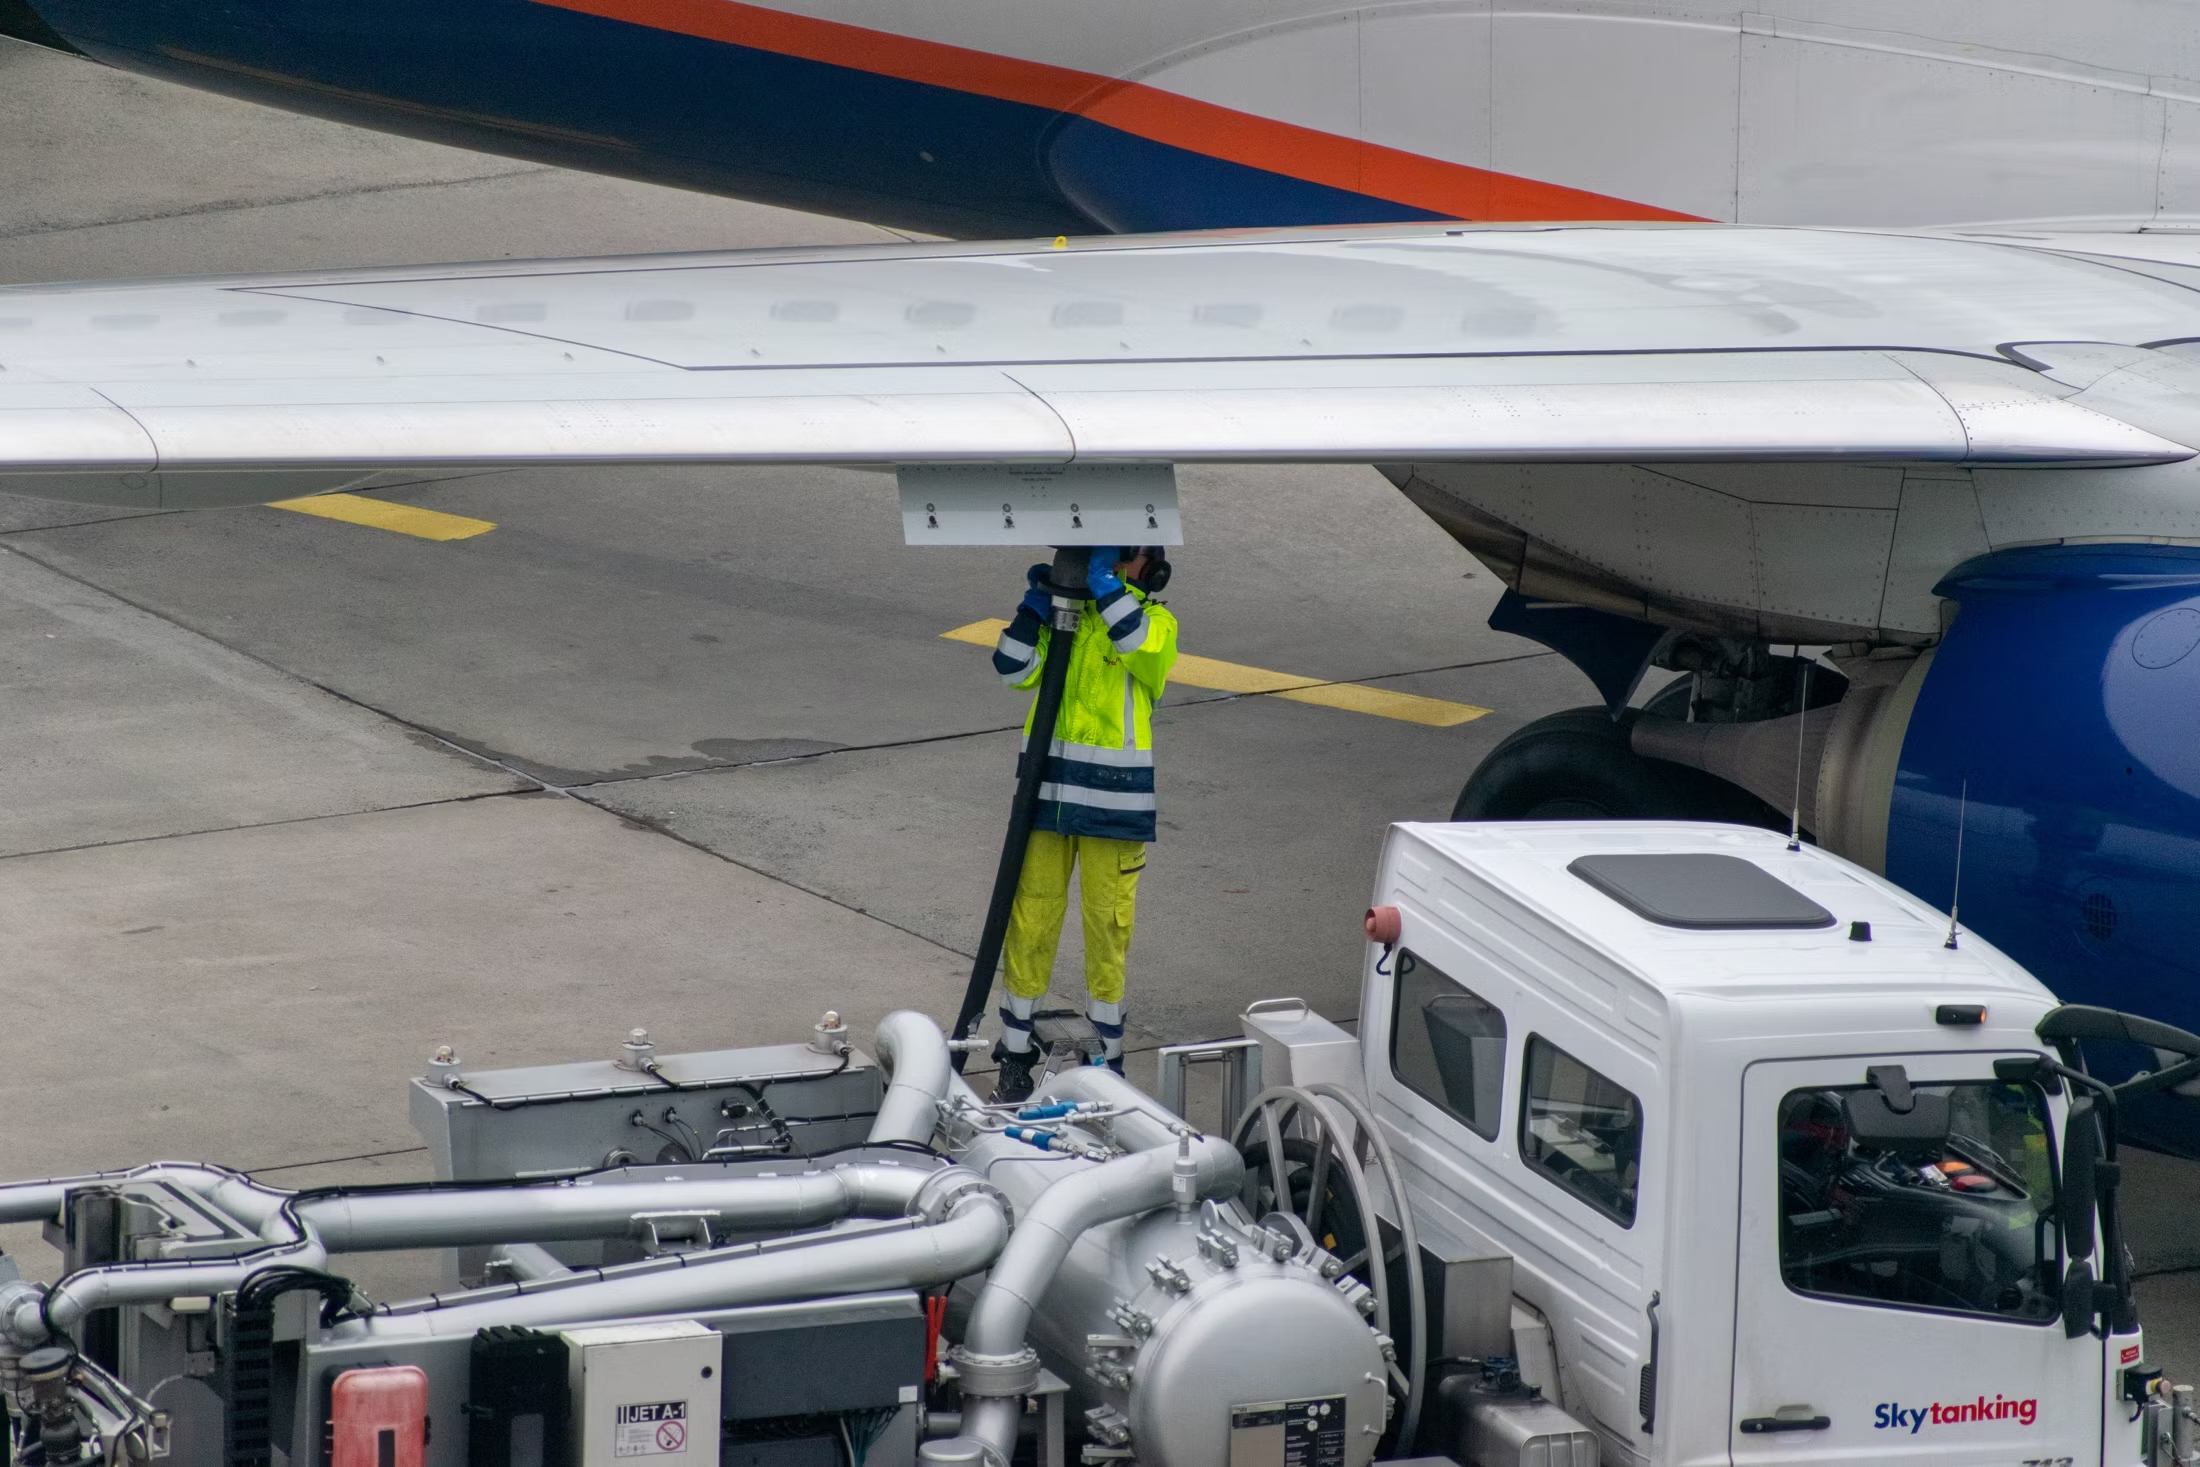
\includegraphics[width=0.5\textwidth]{figures/pressure-refuelling.jpeg}
    \caption{Pressure Refuelling of a Commercial Aircraft. Source: Tom Boon/Simple Flying}\label{fig:pressure-refuelling}
\end{figure}

The aviation industry is undergoing a significant transformation with the
advent of intelligent airports based on highly automated systems. Among these,
automated refuelling systems play a crucial role in ensuring efficient and
accurate refuelling of aircraft. However, one of the main challenges of this
automation process is the accurate detection of the aircraft's refuelling port,
which is relatively small and can easily be obscured by other visual elements
on or near an aircraft. Scanning the entire area of each video frame is both
time-consuming and inaccurate. It is therefore essential to develop a more
efficient and accurate method of locating the refuelling port.

This thesis aims to address this challenge by developing a new AI model that
uses the temporal relationships between successive frames of a video to predict
the location of the refuelling port in subsequent frames. By focusing the
analysis on the most relevant areas of the video sequence, this approach has
the potential to optimise both the speed and accuracy of the refuelling system.

Specific objectives of this thesis include conducting a comprehensive review of
state-of-the-art object detection and tracking methods, designing and
developing a real-time computer vision system capable of accurately detecting
and tracking the pressurised refuelling port of a commercial aircraft, the
implementation and evaluation of deep learning time series models for future
position prediction, the integration of Extended Kalman Filtering (EKF) into
deep learning models to improve the accuracy and robustness of future position
predictions, and the development of a real-time framework for predicting the
future position of the pressurised refuelling port.

By achieving these objectives, this thesis aims to make a significant
contribution to the development of intelligent airport systems and to improve
the efficiency and accuracy of automated refuelling systems at airports, while
reducing computing power requirements. The proposed framework has the potential
to be applied in various scenarios, such as different lighting conditions,
angles and orientations of refuelling ports, making it a versatile and
effective solution to the challenges of automated refuelling systems.
%%%%%%%%%%%%%%%%%%%%%%%%%%%%%%%%%%%%%%%%%%%%%%%%%%%%%%%%%%%%%%%%%%%%%%%%%%%%%%%%

%%%%%%%%%%%%%%%%%%%%%%%%%%%%%%%%%%%%%%%%%%%%%%%%%%%%%%%%%%%%%%%%%%%%%%%%%%%%%%%%
%%%%%%%%%%%%%%%%%%%%%%%%%%%%% LITERATURE REVIEW %%%%%%%%%%%%%%%%%%%%%%%%%%%%%%%%
\chapter{Literature Review}
\section{Automated Refulling Systems in the Aviation Industry}
\subsection{Introduction to Automated Refuelling Systems}
Automated refueling systems have gained substantial importance in the aviation
industry due to their potential to enhance safety and efficiency. The concept
of Autonomous Aircraft Ground Refueling (AAGR) emerged in the 1980s, with
initial implementations featuring numbered markers near refueling ports to aid
in image processing and robotic automation~\cite{Schultz1986, Bennett1991,
    DatasetAGR}.

These systems streamline the refuelling process by using state-of-the-art
mechanisms and technologies to ensure accuracy and speed. A key element is the
pressurised fuel adaptor, which connects seamlessly to the aircraft
~\cite{HybridDatasetAGRV2}. Methods such as `PosEst' have been proposed to
capture and track objects in 3D, enabling the pressurised refuelling port to be
located precisely.~\cite{AGRPoseEstimation}.

In addition, autonomous in-flight refuelling technologies for Unmanned Aerial
Vehicles (UAV-AARs) have also been developed to extend their range, endurance
and payload capacity without significantly altering their original design. This
technology overcomes limitations in fuel capacity and endurance, enabling UAVs
to undertake longer missions~\cite{AARBinocularVision}.

\subsection{Challenges in Automated Refuelling}
The implementation of AAGR presents a number of challenges, including varying
lighting conditions, different refuelling port designs and potential
obstructions. Confidentiality issues associated with aircraft refuelling data,
as well as the lack of standardised workflows, also complicate the deployment
of advanced AAGR solutions, based on~\cite{DatasetAGR} data.

Accurately detecting and estimating the position of the fuelling adaptor is a
major hurdle. Current methods that rely on artificial features often encounter
occlusions and suffer from reduced reliability due to a low signal-to-noise
ratio, particularly over long distances~\cite{AGRPoseEstimation}. Variability
in lighting, weather conditions and the physical state of the refuelling
adapter further complicates detection and
localisation~\cite{HybridDatasetAGRV1}. Vision-based systems must operate in
real time and with minimal computational load, adding a new layer of
complexity.

The development of high-quality data sets for training and monitoring automated
refuelling systems is another major challenge. Collecting and processing these
datasets is often time-consuming and requires meticulous
configuration~\cite{HybridDatasetAGRV2}.

\subsection{Current Technologies and Methods}
Visual measurement methods based on artificial features, such as spray marks or
LEDs, are commonly used in today's automated refuelling systems. The VisNav
system, developed by Valsek, uses light-emitting diodes emitting at different
frequencies to locate the centre of a beacon, employing a Gaussian least
squares differential correction algorithm to calculate the position of
the~\cite{AGRPoseEstimation} refuelling adaptor. Despite the advantages of
these methods, they remain sensitive to occlusion and low signal-to-noise
ratios at long distances.

Recent advances in Automatic Aircraft Ground Refuelling (AAGR) rely on computer
vision, artificial intelligence and robotics to achieve high levels of
automation. The integration of these technologies with Big Data has
significantly improved the feasibility and accuracy of AAGR systems thanks to
the creation of large datasets for training and validation. For example, an
Aircraft Ground Refuelling (AGR) dataset comprising more than 3,000 images from
13 databases was expanded to more than 26,000 images after augmentation,
enabling AGR scene recognition through image mining, augmentation and
classification~\cite{DatasetAGR}. In addition, recent innovations have
introduced hybrid datasets combining real and synthetic data for training and
validating~\cite{HybridDatasetAGRV1} systems. This approach offers a wide range
of scenarios and conditions, improving the robustness and accuracy of automated
refuelling systems.

Furthermore, in the field of autonomous aerial refuelling, current technologies
rely mainly on vision-based systems and sophisticated control algorithms. These
methods use a variety of sensors, including monocular and binocular cameras, to
detect and track drugs and refuelling probes.~\citet{AARCNN} demonstrated the
feasibility of real-time drug recognition and 3D localisation for autonomous
aerial drone refuelling using monocular computer vision. In
addition,~\citet{Chen2011} explored the application of 3D flash lidar for drug
tracking~\cite{AARCNN}. The probe and drogue refuelling system involves the
refuelling aircraft towing a refuelling hose with a drogue at the end, while
the pilot of the receiving aircraft manoeuvres to insert the probe into the
drogue. For unmanned aerial refuelling, this process is carried out
autonomously. Although DGPS offers high location accuracy, it faces challenges
such as lock-in problems and low bandwidth in air-to-air refuelling
applications~\cite{AAREKF}.

\subsection{Future Directions and Innovations}
Future progress in AAGR will depend on systematic research and improvements in
training processes and classifier design. One promising approach is to use
image style transformation technologies based on generative models to simulate
changes in real-world visual conditions such as weather, lighting and camera
angles~\cite{DatasetAGR}. However, these technologies need to be refined to
become specific to aircraft ground refuelling scenarios.

Expanding the training datasets to encompass various aircraft models and
exploring alternative filtering methods to reduce system delays are also key to
future improvements. Ongoing technological developments are expected to
minimise human intervention in refuelling tasks, paving the way for more
efficient and accurate autonomous systems~\cite{AGRPoseEstimation}.

Validation of the results using other measurement methods, such as laser
trackers, and testing of the systems developed on passenger aircraft under real
conditions are essential steps. This research aims to ensure the reliability
and applicability of automated refuelling systems in operational
environments~\cite{HybridDatasetAGRV1}.

Advances in computer vision algorithms and hardware will be key to improving
the accuracy and reliability of position measurements. Innovations in sensor
fusion, combining data from various sources such as vision systems and
Differential Global Positioning Systems (DGPS), could lead to more robust
solutions. Improved real-time image processing capabilities and sophisticated
filtering techniques, such as the Extended Kalman Filter (EKF), are likely to
play a key role in the evolution of autonomous aerial refuelling
technologies~\cite{AAREKF}.

Further integration of advanced computer vision techniques and machine learning
algorithms can significantly improve the accuracy and reliability of the
refuelling process. The development of more sophisticated synthetic datasets
that simulate a wider range of conditions and scenarios will improve the
system's ability to handle real-world variations and
anomalies~\cite{HybridDatasetAGRV2}.

By continually refining these systems, the aviation industry is one step closer
to achieving fully autonomous and highly efficient refuelling operations,
marking an important milestone in intelligent airport operations and advances
in aviation safety.

\section{Object Detection and Tracking in Computer Vision}

\subsection{Fundamentals of Object Detection and Tracking}
Object detection and tracking are fundamental tasks in computer vision,
involving the identification and continuous observation of objects in a video
sequence. Traditional tracking algorithms mainly use visual information to
locate the target by building a model that estimates the similarity between the
target and the search region. However, these models often fail in complex
scenes populated with similar objects, leading to confusion and loss of the
target. Innovations such as the KYS algorithm proposed by \citet{Bhat2020}
incorporate scene information represented as dense localised state vectors,
which are propagated throughout the sequence to provide additional context to
the appearance model. The LaSOT dataset further enhances tracking by providing
linguistic specifications that describe the target and its environment,
conveying valuable semantic information that aids tracking in complex scenes
\cite{SurveyVisualOT}. These advances are crucial for applications such as
automated refuelling systems, intelligent transport and industrial automation,
where accurate object detection and tracking are imperative for efficiency and
safety \cite{OverviewCorrelationAlgoOT, SuveyAdvancesSingleOTMethods}.

\subsection{Algorithms and Techniques for Object Detection}
In the field of object detection, a plethora of algorithms and techniques have
been developed to improve accuracy and robustness. Performance metrics such as
accuracy, robustness, precision, recall and mean accuracy (mAP) are essential
\cite{SurveySmallObjectDetection}. The best-known models for single small
object detection include the fast R-CNN, SSD: Single Shot Multibox Detector,
and YOLO (You Only Look Once), each evaluated on datasets such as Microsoft
COCO and PASCAL VOC \cite{SurveySmallObjectDetection,
    SmallObjectDetectionPositonPrediction, SurveyModernODModels}. Generative
trackers, capable of handling challenging scenarios such as occlusion and
large-scale variation through particle sampling strategies, are often
integrated with various appearance models, including sparse representation and
energy of motion. Discriminative trackers, by contrast, build robust
classifiers using hand-crafted or deep features \cite{SurveyVisualOT}. The
combination of generative and discriminative approaches, as well as the
integration of deep learning techniques such as fully revolutionary networks
and Transformer models, has led to significant improvements in object detection
performance \cite{OverviewCorrelationAlgoOT, SuveyAdvancesSingleOTMethods,
    SurveyModernODModels}. In addition, the speed and computational requirements of
these algorithms are critical factors influencing their practical applicability
\cite{SuveyAdvancesSingleOTMethods, SurveyModernODModels,
    SurveyTransformersSingleOT}.

\subsection{Advanced Techniques for Object Tracking}
Advanced techniques in object tracking leverage both generative and
discriminative models to amplify tracking efficacy. The utilisation of deep
trackers has evidenced superior results on public tracking datasets, attributed
to their potent feature extractors, accurate bounding box regressors, and
discriminative classifiers \cite{SurveyTransformersSingleOT}. Techniques such
as deformable convolution and Transformer models extend traditional convolution
or correlation methodologies to execute global feature matching, thereby
enhancing tracking accuracy. The incorporation of contextual or knowledge
information can substantially elevate performance, with methodologies like
Particle Filtering, also recognised as Sequential Monte Carlo (SMC) methods,
framed as problems of Bayesian inference in state space
\cite{SurveySmallObjectDetection, SmallObjectDetectionPositonPrediction}. The
extended Kalman Filtering (EKF) is another advanced technique that has been
employed to improve tracking accuracy by predicting the current status through
the previous status and modifying the prediction result based on observation
information \cite{SuveyAdvancesSingleOTMethods, SurveyModernODModels}. Despite
these advancements, the integration of these methods in a complementary manner
remains an open research area with substantial potential for advancing the
field \cite{OverviewCorrelationAlgoOT, SuveyAdvancesSingleOTMethods}.

\subsection{Challenges and Future Research Directions}
Despite considerable progress, several challenges persist in the domain of
object detection and tracking. A primary challenge is the integration of
language and visual information to enhance tracking in complex scenes. Semantic
information derived from language specifications can furnish valuable context
that aids trackers in more accurately locating targets \cite{SurveyVisualOT}.
The Drifting Problem, where inaccuracies in foreground and background
estimation degrade the appearance model over time, particularly during
occlusions or imprecise object locations, remains a significant issue.
Additionally, challenges such as motion blurring, limited camera equipment, and
the necessity for real-time processing must be addressed
\cite{OverviewCorrelationAlgoOT}. Future research should emphasise developing
comprehensive large-scale datasets tailored for small object detection, like
SODA-D and SODA-A, focusing on driving and aerial scenarios respectively
\cite{SurveySmallObjectDetection, SmallObjectDetectionPositonPrediction}.
Further, exploring the potential of multi-modal information, enhancing
multi-frame processing techniques such as optical flow estimation for key
frames, and creating adaptive tracking systems capable of adjusting to
appearance variations due to rotations, geometric transformations, and texture
changes, are critical areas for future exploration \cite{SurveyVisualOT,
    OverviewCorrelationAlgoOT, SmallObjectDetectionPositonPrediction,
    SuveyAdvancesSingleOTMethods, SurveyModernODModels,
    SurveyTransformersSingleOT}.

\section{Deep Learning for Spacio-Temporal Prediction}
\subsection{Fundamentals of Time Series Prediction}
Time series prediction involves processing sequential data to predict future
events or values. Various deep learning models have been applied to this task,
requiring several preparatory steps such as collecting data, designating
attribute types, dealing with inconsistencies and storing datasets. These
datasets are usually classified into units of time such as seconds, minutes and
hours, allowing the construction of metadata for machine
learning~\cite{FFPSpaceSystemVehicles}.

The problem of locating future objects has been widely studied, particularly
for static surveillance cameras, from a bird's-eye view. Early work used
recurrent neural networks (RNNs), including long-term memory networks (LSTMs)
and managed recurrent units (GRUs), in an encoder-decoder format to encode past
observations and decode future locations. Additional inputs, such as
environmental information and semantic actions, were used to improve prediction
accuracy.~\citet{Alahi2016} proposed a Social-LSTM to model pedestrian
trajectories and interactions, further improving global context capture through
a social pooling module~\cite{FusionGRU}. Recent advances have taken advantage
of generative models and attention mechanisms to handle complex scenes
involving various interacting agents~\cite{FusionGRU}.

The article of \citet{SpatioTemporalTransformerRecommender} discusses various
deep learning models used to predict time series. In particular, the work
by~\citet{Feng2018} uses attentional recurrent networks to predict human
mobility~\cite{SpatioTemporalTransformerRecommender}. In addition, the paper
highlights the use of BERT4Rec, which exploits bidirectional representations of
transformer encoders for sequential recommendation
tasks~\cite{SpatioTemporalTransformerRecommender}.

Several models for predicting ship trajectories have been proposed. Anderson
considered ship trajectories as a one-dimensional Gaussian process and
predicted smoothed trajectories by combining the dynamics with joint prior
density and covariance matrices.~\citet{Jiang} used a polynomial Kalman filter
for recursive trajectory prediction with minimal memory
usage.~\citet{Zhang2018} adopted a spatial clustering method for prediction,
using the DBSCAN model to cluster and denoise the original AIS trajectories.
Rong introduced a probabilistic model describing the uncertainty of future ship
positions through continuous probability distributions, which achieved high
prediction accuracy~\cite{WaterShipTrajectoryPrediction}.

\subsection{Recurrent Neural Networks and Long Short-Term Memory Networks}
Recurrent neural networks (RNNs), including long-term memory networks (LSTMs)
and managed recurrent units (GRUs), have shown promise for predicting the
future locations of traffic agents~\cite{FusionGRU}. However, many RNN-based
models suffer from performance degradation over time due to their reliance on
recurrent prediction of future bounding boxes from previous outputs. The
Fusion-GRU model addresses these challenges by exploiting multiple sources of
information, such as location scale data, monocular depth information and
optical flow data. This approach improves representation learning by capturing
the complex interactions between the various information cues, thereby
improving the future localisation of traffic agents in congested and risky
driving scenes~\cite{FusionGRU}.

RNNs are powerful for processing sequence information and making time-based
predictions. Hochreiter et al. improved the structure of the RNN unit,
introducing the LSTM model to solve the problems of gradient fading, gradient
explosion and insufficient information memory through a
gating~\cite{WaterShipTrajectoryPrediction} mechanism. LSTMs make efficient use
of long-range temporal information, which is useful in a variety of prediction
tasks. However, BP neural networks and SVMs also exist for trajectory
prediction, but have limitations such as weaker handling of non-linear problems
and susceptibility to local extrema~\cite{WaterShipTrajectoryPrediction}.

\subsection{Transformer models for sequence prediction}
Recent research has used transform-based methods for estimating the future
location of traffic~cite{FusionGRU} agents. Despite advances in deep learning
for locating objects in typical driving scenarios, predicting locations in
risky scenarios remains challenging due to abrupt changes in motion and
interdependencies between successive images~\cite{FusionGRU}.

The Transformer model, introduced by~\citet{Vaswani2017}, has revolutionised
sequence modelling with its efficient and powerful network structure. For
mobility prediction, Transformer models are increasingly recognised for
addressing the challenges of predicting individual mobility patterns.
The~\citet{HowDoUGoWhere} study shows how transformers can effectively learn
mobility patterns from historical data, achieving state-of-the-art performance
in next-location prediction tasks.

Further validation and extensive experiments on real-world datasets affirm
their efficacy in improving prediction accuracy. The work
of~\citet{SpatioTemporalTransformerRecommender} discusses the application of
transformers and self-attention mechanisms in sequence prediction, highlighting
their effectiveness in various contexts.

\subsection{Challenges and Future Research Directions}
Despite significant advances, several challenges persist in deep learning
models for time series prediction. One of the main challenges is the
performance degradation of RNN-based models over time, addressed by models such
as Fusion-GRU, which exploit multiple data sources for better
representation~\cite{FusionGRU}. Accurate prediction in risky driving
scenarios, involving sudden or abrupt changes in motion, is still unresolved.
Future research could focus on improving model robustness in these scenarios
and integrating additional data sources to improve prediction
accuracy~\cite{FusionGRU}.

The article of~\citet{MLTechniqueFPP} identifies several challenges in location
prediction using machine learning, highlighting the need for trajectory data
quality and extensive pre-processing. Future research could incorporate
semantic information to improve prediction accuracy, taking advantage of
ensemble techniques and overcoming data limitations. The ensemble architecture
recommended in the paper shows a significant reduction in mean distance error
compared to reference models~\cite{MLTechniqueFPP}.

%% Back matter
%
% This is where we include references and appendices

\bibliographystyle{abbrvnat}
\bibliography{LaTeX,CUCitations}

\appendix
\chapter{Ethical Approval Letter}
Insert your Ethical Approval Letter as the first appendix.

\chapter{Extra Data}
This is a sample of thesis text. This is a sample of thesis text. This is a
sample of thesis text. This is a sample of thesis text. This is a sample of
thesis text.

This is a sample of thesis text. This is a sample of thesis text. This is a
sample of thesis text. This is a sample of thesis text. This is a sample of
thesis text.

\end{document}

